\documentclass{beamer}
\usepackage{graphicx}
\usepackage{graphics}
\usepackage{hyperref}
\usepackage[english]{babel}

\mode<presentation>
{
    \usetheme{AMUFree-kk}
    \setbeamercovered{transparent = 28}
}
\title{\normalsize{Unsupervised learning methods based on huge data for the needs of supervised learning methods using small training sets}}
\author[{K. Kaczmarek}]{Karol Kaczmarek}
\date{2018}
\setbeamertemplate{bibliography item}{[\theenumiv]}

\begin{document}

\begin{frame}
    \titlepage
\end{frame}

\AtBeginSection[]
{
    \begin{frame}
        \frametitle{Outline}
        \tableofcontents[currentsection]
    \end{frame}
}


\section{Difficulties}

\begin{frame}
    \frametitle{Difficulties}
    \begin{itemize}
        \item supervised learning methods using small training sets
        \begin{itemize}
            \item classification
            \item extraction
        \end{itemize}
      \item increasing the amount of small training sets
      \item noisy data (types, ORC error, rare words)
      \item unbalanced training sets
      \item time and costs
    \end{itemize}
\end{frame}

\section{Neural language model}

\begin{frame}
    \frametitle{Neural language model}
    \begin{itemize}
        \item use different architectures:
        \begin{itemize}
            \item word level
            \item char level
            \item sentence level
        \end{itemize}
        \item evaluation models:
        \begin{itemize}
            \item perplexity
            \item guest gap
        \end{itemize}
        \item OCR types tolerant
    \end{itemize}
\end{frame}

\begin{frame}
    \frametitle{Neural language model}
    \begin{itemize}

        \item use embedding of models:
        \begin{itemize}
            \item CoVe \cite{CoVe}
            \item ELMo \cite{ELMo}
            % \item Transformers
            % \item Flair
            % \item Universal Sentence Encoder
        \end{itemize}
        \item compare with:
        \begin{itemize}
            % \item Glove
            \item word2vec \cite{word2vec}
            \item fastText \cite{fastText}
        \end{itemize}
    \end{itemize}
\end{frame}

\begin{frame}
    \frametitle{CoVe}
    \begin{itemize}
        \item inspired by the pretrained ImageNet
        \item train an encoder and transfer the encoder to other tasks
        \item training an attentional sequence-to-sequence model for English-to-German translation
        \begin{center}
            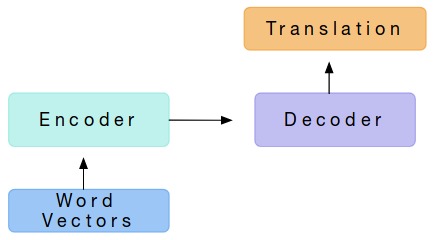
\includegraphics{img/CoVe-encoder.png}
        \end{center}
        \item $ CoVe(w) = MT$-$LSTM(GloVe(w))$, $w$ - sequence of words
    \end{itemize}
\end{frame}

\begin{frame}
    \frametitle{CoVe}
    \begin{center}
        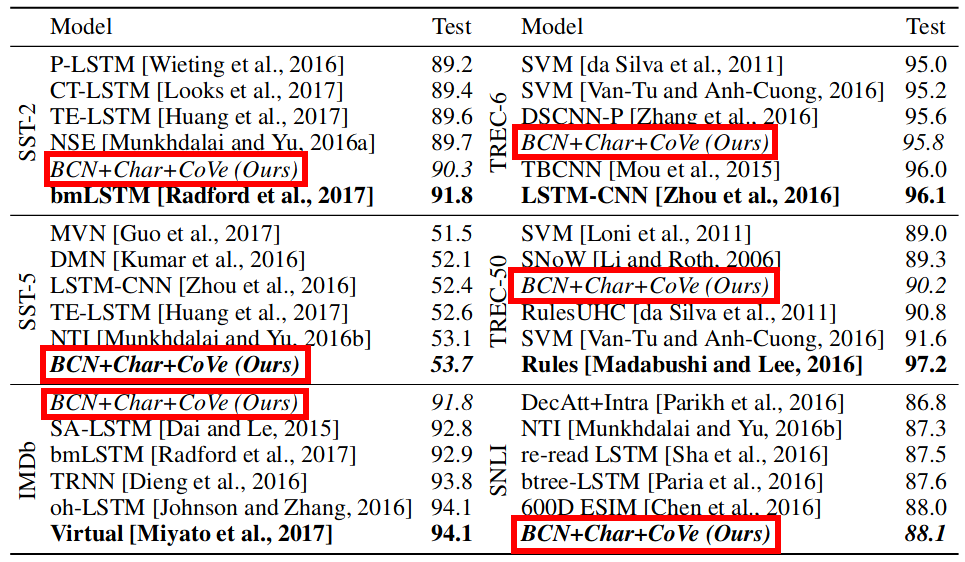
\includegraphics{img/CoVe-result.png}
    \end{center}
\end{frame}

\begin{frame}
    \frametitle{ELMo (Embeddings from Language Models)}
    \begin{itemize}
        \item function of all of the internal layers of the biLM
        \item lower-level LSTM states model aspects of syntax
        \item higher-level LSTM states capture context-dependent aspects of  word meaning
        \item ELMo outperforms CoVe
    \end{itemize}
\end{frame}

\begin{frame}
    \frametitle{ELMo (Embeddings from Language Models)}
    \begin{center}
        \includegraphics{img/ELmo-result.png}
    \end{center}
\end{frame}

\section{Data sets}

\begin{frame}
    \frametitle{Data sets}
    \begin{itemize}
        \item Get more data
        \begin{itemize}
            \item Common Crawl
            \item Wikipedia
        \end{itemize}
    \item Extract in-domain data sets
    \item Data augmentation
    \end{itemize}
\end{frame}


% References
\section{References}
\begin{frame}[allowframebreaks,t]
    \tiny
    \frametitle{References}
    \bibliographystyle{ieeetr}
    \bibliography{kk_phd}
    %\nocite{*}
\end{frame}

\end{document}
